\chapter{PX4}
\section{编译}
对于简单的工程,可以直接手动用gcc/g++将.c/.cpp文件编译链接为可执行文件。若工程包含多个文件夹多个文件,可以通过编写makefile文件并利用make工具,自动化地对所有文件进行编译。而对于更为复杂的工程,可以通过编写CMakeLists文件,并利用cmake工具,自动化地生成makefile文件。

PX4代码编译的入口是根目录下的Makefile文件。该Makefile文件首先执行一些基本的检测、设置,然后利用cmake工具,由根目录下的CMakeLists文件和PX4代码结构中的其他配置文件,自动生成makefile文件并进行make编译。

make命令的基本教程可以参考\href{http://www.ruanyifeng.com/blog/2015/02/make.html}{这里}。

首先对git环境、编译工具、系统目录等进行了简单的检测和配置:
\begin{lstlisting}[language=make,numbers=left,firstnumber = 38,numberstyle=\tiny,breaklines = true,keywordstyle=\color{blue!70},commentstyle=\color{red!50!green!50!blue!50},frame=shadowbox, rulesepcolor=\color{red!20!green!20!blue!20}]
	ifeq ($(wildcard .git),)
    $(error YOU HAVE TO USE GIT TO DOWNLOAD THIS REPOSITORY. ABORTING.)
endif

CMAKE_VER := $(shell Tools/check_cmake.sh; echo $$?)
ifneq ($(CMAKE_VER),0)
    $(warning Not a valid CMake version or CMake not installed.)
    $(warning On Ubuntu 16.04, install or upgrade via:)
    $(warning )
    $(warning 3rd party PPA:)
    $(warning sudo add-apt-repository ppa:george-edison55/cmake-3.x -y)
    $(warning sudo apt-get update)
    $(warning sudo apt-get install cmake)
    $(warning )
    $(warning Official website:)
    $(warning wget https://cmake.org/files/v3.4/cmake-3.4.3-Linux-x86_64.sh)
    $(warning chmod +x cmake-3.4.3-Linux-x86_64.sh)
    $(warning sudo mkdir /opt/cmake-3.4.3)
    $(warning sudo ./cmake-3.4.3-Linux-x86_64.sh --prefix=/opt/cmake-3.4.3 --exclude-subdir)
    $(warning export PATH=/opt/cmake-3.4.3/bin:$$PATH)
    $(warning )
    $(error Fatal)
endif
\end{lstlisting}

\begin{lstlisting}[language=make,numbers=left,firstnumber = 79,numberstyle=\tiny,breaklines = true,keywordstyle=\color{blue!70},commentstyle=\color{red!50!green!50!blue!50},frame=shadowbox, rulesepcolor=\color{red!20!green!20!blue!20}]
#  explicity set default build target
all: posix_sitl_default

# Parsing
# --------------------------------------------------------------------
# assume 1st argument passed is the main target, the
# rest are arguments to pass to the makefile generated
# by cmake in the subdirectory
FIRST_ARG := $(firstword $(MAKECMDGOALS))
ARGS := $(wordlist 2,$(words $(MAKECMDGOALS)),$(MAKECMDGOALS))
j ?= 4

ifndef NO_NINJA_BUILD
NINJA_BUILD := $(shell ninja --version 2>/dev/null)
endif
ifdef NINJA_BUILD
    PX4_CMAKE_GENERATOR ?= "Ninja"
    PX4_MAKE = ninja
    PX4_MAKE_ARGS =
else

ifdef SYSTEMROOT
	# Windows
	PX4_CMAKE_GENERATOR ?= "MSYS Makefiles"
else
	PX4_CMAKE_GENERATOR ?= "Unix Makefiles"
endif
    PX4_MAKE = $(MAKE)
    PX4_MAKE_ARGS = -j$(j) --no-print-directory
endif

# check if replay env variable is set & set build dir accordingly
ifdef replay
	BUILD_DIR_SUFFIX := _replay
else
	BUILD_DIR_SUFFIX :=
endif

# additional config parameters passed to cmake
CMAKE_ARGS :=
ifdef EXTERNAL_MODULES_LOCATION
	CMAKE_ARGS := -DEXTERNAL_MODULES_LOCATION:STRING=$(EXTERNAL_MODULES_LOCATION)
endif

SRC_DIR := $(shell dirname $(realpath $(lastword $(MAKEFILE_LIST))))
\end{lstlisting}

以下是/cmake/configs/目录下获取所有可编译的目标,其中ALL_CONFIG_TARGETS是所有目标,NUTTX_CONFIG_TARGETS是NUTTX_开头的目标。
\begin{lstlisting}[language=make,numbers=left,firstnumber = 149,numberstyle=\tiny,breaklines = true,keywordstyle=\color{blue!70},commentstyle=\color{red!50!green!50!blue!50},frame=shadowbox, rulesepcolor=\color{red!20!green!20!blue!20}]
# Get a list of all config targets.
ALL_CONFIG_TARGETS := $(basename $(shell find "$(SRC_DIR)/cmake/configs" ! -name '*_common*' ! -name '*_sdflight_*' -name '*.cmake' -print | sed  -e 's:^.*/::' | sort))
# Strip off leading nuttx_
NUTTX_CONFIG_TARGETS := $(patsubst nuttx_%,%,$(filter nuttx_%,$(ALL_CONFIG_TARGETS)))
\end{lstlisting}

然后利用call-build对当前目标(\$@)进行编译。再往下基本都是各种伪目标的说明。
\begin{lstlisting}[language=make,numbers=left,firstnumber = 158,numberstyle=\tiny,breaklines = true,keywordstyle=\color{blue!70},commentstyle=\color{red!50!green!50!blue!50},frame=shadowbox, rulesepcolor=\color{red!20!green!20!blue!20}]
	# All targets.
	$(ALL_CONFIG_TARGETS):
		$(call cmake-build,$@)
	
	# Abbreviated config targets.
	
	# nuttx_ is left off by default; provide a rule to allow that.
	$(NUTTX_CONFIG_TARGETS):
		$(call cmake-build,nuttx_$@)
\end{lstlisting}

对cmake-build的宏定义是Makefile文件中的核心部分:
\begin{lstlisting}[language=make,numbers=left,firstnumber = 125,numberstyle=\tiny,breaklines = true, keywordstyle=\color{blue!70},commentstyle=\color{red!50!green!50!blue!50},frame=shadowbox, rulesepcolor=\color{red!20!green!20!blue!20}]
# Functions
# --------------------------------------------------------------------
# describe how to build a cmake config
define cmake-build
+@$(eval BUILD_DIR = $(SRC_DIR)/build_$@$(BUILD_DIR_SUFFIX))
+@if [ $(PX4_CMAKE_GENERATOR) = "Ninja" ] && [ -e $(BUILD_DIR)/Makefile ]; then rm -rf $(BUILD_DIR); fi
+@if [ ! -e $(BUILD_DIR)/CMakeCache.txt ]; then mkdir -p $(BUILD_DIR) && cd $(BUILD_DIR) && cmake .. -G$(PX4_CMAKE_GENERATOR) -DCONFIG=$(1) $(CMAKE_ARGS) || (cd .. && rm -rf $(BUILD_DIR)); fi
+@echo "PX4 CONFIG: $(BUILD_DIR)"
+@$(PX4_MAKE) -C "$(BUILD_DIR)" $(PX4_MAKE_ARGS) $(ARGS)
endef
\end{lstlisting}

129行定义BUILD_DIR = /build_\$@变量,也就是之后所有编译文件生成的目录。130行判断Ninja和cmake之间的冲突。

131行首先根据BUILD_DIR/CMakeCache.txt文件来判断是否需要创建BUILD_DIR文件夹并调用cmake。cmake .. 是指根据根目录下的CMakeLists进行makefile文件生成,-G\$(PX4_CMAKE_GENERATOR)则是指定使用Ninja或是cmake,-DCONFIG=\$(1)是将第一个参数赋值给cmake的变量CONFIG,该变量在CMakeLists中指定了生成makefile文件过程中会包含哪个cmake/configs/.cmake文件。

133行,根据目标目录下的makefile文件(或是Ninja的rule文件)编译。

如果想屏蔽掉Ninja,可以在91行之前添加宏定义:
\begin{lstlisting}[language=make,numbers=left,firstnumber = 0,breaklines = true,numberstyle=\tiny,keywordstyle=\color{blue!70},commentstyle=\color{red!50!green!50!blue!50},frame=shadowbox, rulesepcolor=\color{red!20!green!20!blue!20}]
define NO_NINJA_BUILD
endef
\end{lstlisting}



\section{软件在环仿真SIL}
\subsection{启动流程}
以下用 make posix_sitl_default jmavsim 为例,分析软件在环仿真(SITL)启动流程。

编译完posix_sitl_default目标后,会调用/Tools/sitl_run.sh脚本(通过什么调用的还不知道)。
\begin{lstlisting}[language=bash,numbers=left,firstnumber = 1,breaklines = true,numberstyle=\tiny,keywordstyle=\color{blue!70},commentstyle=\color{red!50!green!50!blue!50},frame=shadowbox, rulesepcolor=\color{red!20!green!20!blue!20}]
#!/bin/bash

set -e

echo args: $@

sitl_bin=$1
rcS_dir=$2
debugger=$3
program=$4
model=$5
src_path=$6
build_path=$7

echo SITL ARGS

echo sitl_bin: $sitl_bin
echo rcS_dir: $rcS_dir
echo debugger: $debugger
echo program: $program
echo model: $model
echo src_path: $src_path
echo build_path: $build_path

working_dir=`pwd`
sitl_bin=$build_path/src/firmware/posix/px4
rootfs=$build_path/tmp/rootfs

if [ "$chroot" == "1" ]
then
	chroot_enabled=-c
	sudo_enabled=sudo
else
	chroot_enabled=""
	sudo_enabled=""
fi

# To disable user input
if [[ -n "$NO_PXH" ]]; then
	no_pxh=-d
else
	no_pxh=""
fi

if [ "$model" == "" ] || [ "$model" == "none" ]
then
	echo "empty model, setting iris as default"
	model="iris"
fi

if [ "$#" -lt 7 ]
then
	echo usage: sitl_run.sh rc_script rcS_dir debugger program model src_path build_path
	echo ""
	exit 1
fi

# kill process names that might stil
# be running from last time
pgrep gazebo && pkill gazebo
pgrep px4 && pkill px4
jmavsim_pid=`ps aux | grep java | grep Simulator | cut -d" " -f1`
if [ -n "$jmavsim_pid" ]
then
	kill $jmavsim_pid
fi

cp $src_path/Tools/posix_lldbinit $working_dir/.lldbinit
cp $src_path/Tools/posix.gdbinit $working_dir/.gdbinit

SIM_PID=0

if [ "$program" == "jmavsim" ] && [ ! -n "$no_sim" ]
then
	$src_path/Tools/jmavsim_run.sh &
	SIM_PID=`echo $!`
	cd ../..
elif [ "$program" == "gazebo" ] && [ ! -n "$no_sim" ]
then
	if [ -x "$(command -v gazebo)" ]
	then
		# Set the plugin path so Gazebo finds our model and sim
		source $src_path/Tools/setup_gazebo.bash ${src_path} ${build_path}

		gzserver --verbose ${src_path}/Tools/sitl_gazebo/worlds/${model}.world &
		SIM_PID=`echo $!`

		if [[ -n "$HEADLESS" ]]; then
			echo "not running gazebo gui"
		else
			gzclient --verbose &
			GUI_PID=`echo $!`
		fi
	else
		echo "You need to have gazebo simulator installed!"
		exit 1
	fi
elif [ "$program" == "replay" ] && [ ! -n "$no_sim" ]
then
	echo "Replaying logfile: $logfile"
	# This is not a simulator, but a log file to replay

	# Check if we need to creat a param file to allow user to change parameters
	if ! [ -f "$rootfs/replay_params.txt" ]
		then
		mkdir -p $rootfs
		touch $rootfs/replay_params.txt
	fi
fi

cd $working_dir

if [ "$logfile" != "" ]
then
	cp $logfile $rootfs/replay.px4log
fi

# Do not exit on failure now from here on because we want the complete cleanup
set +e

sitl_command="$sudo_enabled $sitl_bin $no_pxh $chroot_enabled $src_path $src_path/${rcS_dir}/${model}"

echo SITL COMMAND: $sitl_command

# Start Java simulator
if [ "$debugger" == "lldb" ]
then
	lldb -- $sitl_command
elif [ "$debugger" == "gdb" ]
then
	gdb --args $sitl_command
elif [ "$debugger" == "ddd" ]
then
	ddd --debugger gdb --args $sitl_command
elif [ "$debugger" == "valgrind" ]
then
	valgrind $sitl_command
else
	$sitl_command
fi

if [ "$program" == "jmavsim" ]
then
	pkill -9 -P $SIM_PID
	kill -9 $SIM_PID
elif [ "$program" == "gazebo" ]
then
	kill -9 $SIM_PID
	if [[ ! -n "$HEADLESS" ]]; then
		kill -9 $GUI_PID
	fi
fi
\end{lstlisting}
其中,73行判断仿真器,如果是jmavsim,则在75行调用/Tools/jmavsim_run.sh,启动仿真器。在jmavsim_run.sh中,主要是在最后先进行编译,然后执行仿真器:
\begin{lstlisting}[language=bash,numbers=left,firstnumber = 37,breaklines = true,numberstyle=\tiny,keywordstyle=\color{blue!70},commentstyle=\color{red!50!green!50!blue!50},frame=shadowbox, rulesepcolor=\color{red!20!green!20!blue!20}]
ant create_run_jar copy_res
cd out/production
java -Djava.ext.dirs= -jar jmavsim_run.jar $device $extra_args
\end{lstlisting}
如果是手动启动的话,按照\href{http://www.pixhawk.com/dev/hil/jmavsim#hardware_in_the_loop_hitl}{官网说明},采用如下命令:
\begin{lstlisting}[language=bash,numbers=left,firstnumber = 1,breaklines = true,numberstyle=\tiny,keywordstyle=\color{blue!70},commentstyle=\color{red!50!green!50!blue!50},frame=shadowbox, rulesepcolor=\color{red!20!green!20!blue!20}]
cd ~/jMAVSim
java -Djava.ext.dirs= -cp lib/*:out/production/jmavsim.jar me.drton.jmavsim.Simulator -udp 127.0.0.1:14560   
\end{lstlisting} 
可以看出,对应调用的入口是Simulator.java。

继续在sitl_run.sh中的139行,调用编译出的px4可执行文件,对应在终端中显示的信息示例为:
\begin{lstlisting}[language=bash,numbers=left,firstnumber = 0,breaklines = true,numberstyle=\tiny,keywordstyle=\color{blue!70},commentstyle=\color{red!50!green!50!blue!50},frame=shadowbox, rulesepcolor=\color{red!20!green!20!blue!20}]
SITL COMMAND: /home/zhangbo39/firmware/build_posix_sitl_default/src/firmware/posix/px4 /home/zhangbo39/firmware /home/zhangbo39/firmware/posix-configs/SITL/init/lpe/iris
data path: /home/zhangbo39/firmware
commands file: /home/zhangbo39/firmware/posix-configs/SITL/init/lpe/iris
\end{lstlisting}
其中,SITL COMMAND所显示的也就是手动启动时的命令。

\subsection{jMAVSim 初始化}
jMAVSim中所有的类都包含在World这个类中,其中实例化了的类:

1. SimpleEnvironment, 环境类,包含了对环境风的简单建模;

2. connHIL,通信类,负责仿真系统与PX4之间的通信;

3. connCommon,通信类,负责地面站与PX4之间的通信;

4. vehicle,飞行器类,对仿真对象的简单建模;

5. 视景类(待定)

除此之外,还有1个仿真系统类和2个端口类被实例化,分别是:

1. hilSystem, 仿真系统

2. autopilotMAVLinkPort,飞控通信端口

3. udpGCMAVLinkPort, 地面站通信端口

上述三个端口(系统),1和2被加入到connHIL中,2和3被加入到connCommon中。从这一点可以看出,从飞控端发来的信号除了被送入仿真系统中外,还会被送入地面站。

\subsection{PX4 SITL 初始化}
执行SITL仿真时,入口的启动文件就是命令行的第二个参数,"/home/zhangbo39/firmware/posix-configs/SITL/init/lpe/iris",这个类似与常规的rcS文件。
\begin{lstlisting}[language=bash,numbers=left,firstnumber = 1,breaklines = true,numberstyle=\tiny,keywordstyle=\color{blue!70},commentstyle=\color{red!50!green!50!blue!50},frame=shadowbox, rulesepcolor=\color{red!20!green!20!blue!20}]
uorb start
param load
param set MAV_TYPE 2
param set SYS_AUTOSTART 4010
param set SYS_RESTART_TYPE 2
dataman start
param set BAT_N_CELLS 3
param set CAL_GYRO0_ID 2293768
param set CAL_ACC0_ID 1376264
param set CAL_ACC1_ID 1310728
param set CAL_MAG0_ID 196616
param set CAL_GYRO0_XOFF 0.01
param set CAL_ACC0_XOFF 0.01
param set CAL_ACC0_YOFF -0.01
param set CAL_ACC0_ZOFF 0.01
param set CAL_ACC0_XSCALE 1.01
param set CAL_ACC0_YSCALE 1.01
param set CAL_ACC0_ZSCALE 1.01
param set CAL_ACC1_XOFF 0.01
param set CAL_MAG0_XOFF 0.01
param set SENS_BOARD_ROT 0
param set SENS_BOARD_X_OFF 0.000001
param set COM_RC_IN_MODE 1
param set NAV_DLL_ACT 2
param set COM_DISARM_LAND 3
param set NAV_ACC_RAD 2.0
param set COM_OF_LOSS_T 5
param set COM_OBL_ACT 2
param set COM_OBL_RC_ACT 0
param set RTL_RETURN_ALT 30.0
param set RTL_DESCEND_ALT 5.0
param set RTL_LAND_DELAY 5
param set MIS_TAKEOFF_ALT 2.5
param set MC_ROLLRATE_P 0.2
param set MC_PITCHRATE_P 0.2
param set MC_PITCH_P 6
param set MC_ROLL_P 6
param set MPC_HOLD_MAX_Z 2.0
param set MPC_HOLD_XY_DZ 0.1
param set MPC_Z_VEL_P 0.6
param set MPC_Z_VEL_I 0.15
param set EKF2_GBIAS_INIT 0.01
param set EKF2_ANGERR_INIT 0.01
replay tryapplyparams
simulator start -s
rgbledsim start
tone_alarm start
gyrosim start
accelsim start
barosim start
adcsim start
gpssim start
pwm_out_sim mode_pwm
sleep 1
sensors start
commander start
land_detector start multicopter
navigator start
attitude_estimator_q start
local_position_estimator start
mc_pos_control start
mc_att_control start
mixer load /dev/pwm_output0 ROMFS/px4fmu_common/mixers/quad_w.main.mix
mavlink start -u 14556 -r 4000000
mavlink start -u 14557 -r 4000000 -m onboard -o 14540
mavlink stream -r 50 -s POSITION_TARGET_LOCAL_NED -u 14556
mavlink stream -r 50 -s LOCAL_POSITION_NED -u 14556
mavlink stream -r 50 -s GLOBAL_POSITION_INT -u 14556
mavlink stream -r 50 -s ATTITUDE -u 14556
mavlink stream -r 50 -s ATTITUDE_QUATERNION -u 14556
mavlink stream -r 50 -s ATTITUDE_TARGET -u 14556
mavlink stream -r 50 -s SERVO_OUTPUT_RAW_0 -u 14556
mavlink stream -r 20 -s RC_CHANNELS -u 14556
mavlink stream -r 250 -s HIGHRES_IMU -u 14556
mavlink stream -r 10 -s OPTICAL_FLOW_RAD -u 14556
logger start -e -t
mavlink boot_complete
replay trystart
\end{lstlisting}
上述代码中,45--53行、63行都是与仿真相关的几个文件。simulator应用相当于仿真中的一个底层接口,主要作用是负责接收解析仿真器发来的msg,并将PX4的飞行控制量PWM发送出去。gyrosim、accelsim、barosim、adcsim、gpssim是虚拟的底层传感器,但是数据本质上是从simulator的数据基础上进行了一次转发。pwm_out_sim则是调用混控将飞控控制量计算为PWM值。mixer与仿真相关的地方在于load后的设备参数。

\subsubsection{simulator 模块流程}
\noindent 
/firmware/build_posix_sitl_default/src/firmware/posix/apps.cpp中对应入口函数为
\begin{lstlisting}[language=c++,numbers=left,firstnumber = 1,breaklines = true,numberstyle=\tiny,keywordstyle=\color{blue!70},commentstyle=\color{red!50!green!50!blue!50},frame=shadowbox, rulesepcolor=\color{red!20!green!20!blue!20}]
int simulator_main(int argc, char *argv[])
\end{lstlisting}
启动\texttt{Simulator::start}线程:
\begin{lstlisting}[language=c++,numbers=left,firstnumber = 1,breaklines = true,numberstyle=\tiny,keywordstyle=\color{blue!70},commentstyle=\color{red!50!green!50!blue!50},frame=shadowbox, rulesepcolor=\color{red!20!green!20!blue!20}]
int Simulator::start(int argc, char *argv[]){
	_instance = new Simulator(); //实例化PX4仿真层
	if (_instance) {
		...
		if (argv[2][1] == 's') {
			_instance->initializeSensorData();
#ifndef __PX4_QURT
			// Update sensor data
			_instance->pollForMAVLinkMessages(false, udp_port); 
#endif
		...
{\end{lstlisting}
其中\texttt{_instance->pollForMAVLinkMessages(false, udp_port)}负责仿真阶段的数据收发。具体分为三个阶段:

\noindent (1)阻塞等待UDP数据,每当收到仿真器数据时,回复心跳包。如果收到的数据是非\#0的msg,则进入第二阶段。

\noindent (2)订阅PWM输出、飞机状态消息,创建\texttt{Simulator::sending_trampoline}线程。向仿真器发送\#76消息。进入第三阶段

\noindent (3)阻塞等待UDP数据,每当收到仿真器数据时进行解包,若是特定消息(HIL_SENSOR、HIL_OPTICAL_FLOW、DISTANCE_SENSOR、HIL_GPS、RC_CHANNELS、HIL_STATE_QUATERNION)则进一步更新虚拟传感器数据,将数据写到指定地址。\hhl{特别需要注意的是},此阶段中publish形参传入的参数是false,所以simulator收到的数据并不会直接publish出去,还需要虚拟传感器的中间环节。

\texttt{Simulator::sending_trampoline}的主要流程是阻塞等待_actuator_outputs_sub[0]的更新,然后调用poll_topics()拷贝数据,调用send_controls()函数将数据用\#93消息(HIL_ACTUATOR_CONTROLS)发送出去。

\subsubsection{gyrosim等虚拟传感器 模块流程}
类似地,入口函数为
\begin{lstlisting}[language=c++,numbers=left,firstnumber = 1,breaklines = true,numberstyle=\tiny,keywordstyle=\color{blue!70},commentstyle=\color{red!50!green!50!blue!50},frame=shadowbox, rulesepcolor=\color{red!20!green!20!blue!20}]
int gyrosim_main(int argc, char *argv[])
\end{lstlisting}
启动int start(enum Rotation rotation):
\begin{lstlisting}[language=c++,numbers=left,firstnumber = 1,breaklines = true,numberstyle=\tiny,keywordstyle=\color{blue!70},commentstyle=\color{red!50!green!50!blue!50},frame=shadowbox, rulesepcolor=\color{red!20!green!20!blue!20}]
...
*g_dev_ptr = new GYROSIM(path_accel, path_gyro, rotation);
...
if (OK != (*g_dev_ptr)->init()) {
	goto fail;
}
...
\end{lstlisting}
之后都会调用_measure()函数,在其中通过执行如下函数读取simulator的数据。
\begin{lstlisting}[language=c++,numbers=left,firstnumber = 1,breaklines = true,numberstyle=\tiny,keywordstyle=\color{blue!70},commentstyle=\color{red!50!green!50!blue!50},frame=shadowbox, rulesepcolor=\color{red!20!green!20!blue!20}]
if (OK != transfer((uint8_t *)&mpu_report, ((uint8_t *)&mpu_report), sizeof(mpu_report))) {
	return;
}
\end{lstlisting}
在transfer()函数中,实例化一个临时的Simulator并调用getMPUReport()读取数据,然后回传数据。

从代码中可以看出,gyrosim、accelsim会读取并发布多个传感器的数据,具体如下:

\noindent gyrosim: gyro(优先级HIGH,100),accel(优先级HIGH,100)

\noindent accelsim: accel(优先级DEFAULT,75),mag(优先级LOW,50)

另外,如果将gyrosim应用屏蔽掉,则仿真中sensors status的四个传感器通道数据都是-1。这时因为在sensors模块中,更新数据是阻塞等待gyro数据,所以如果改为阻塞等待accel数据,则另外三个通道数据都会出现,但是accel只有75优先级的数据。
\begin{figure}[htbp]
	\figskip
	\centering
	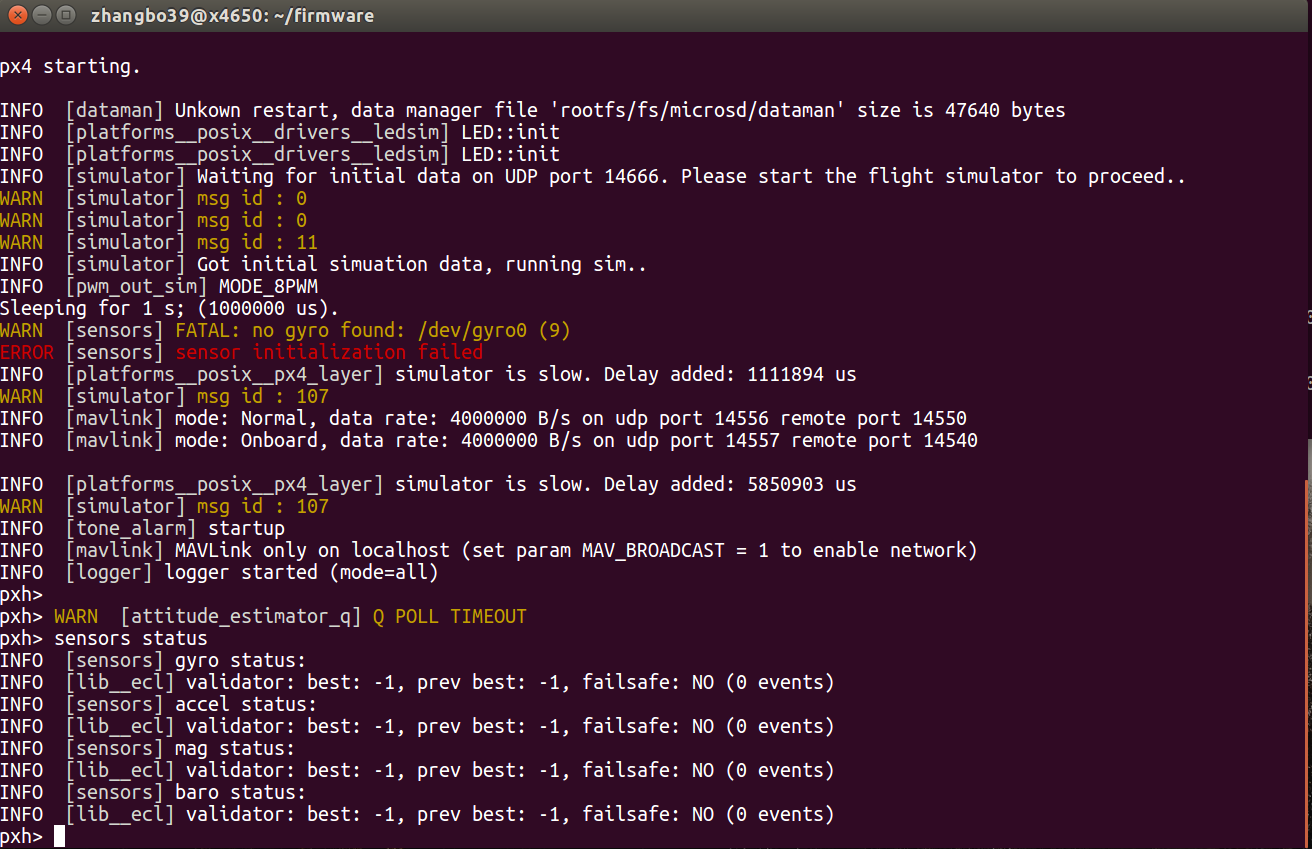
\includegraphics[width = \textwidth,trim = 0 -0 0 -0,clip]{sensors01.png}	  
	\caption{\label{fig: 1} 阻塞等待gyro数据时屏蔽gyrosim}
\end{figure}

\begin{figure}[htbp]
	\figskip
	\centering
	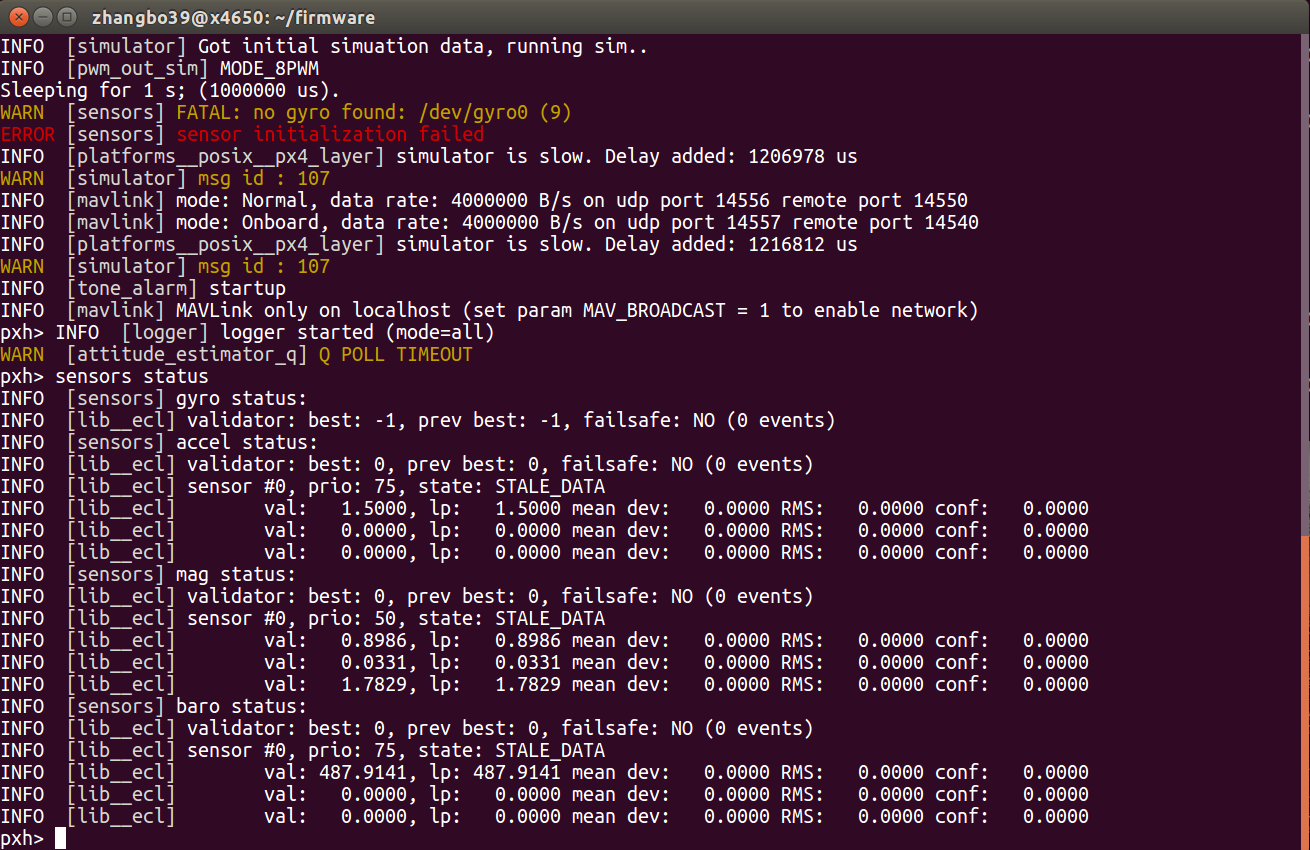
\includegraphics[width = \textwidth,trim = 0 -0 0 -0,clip]{sensors02.png}	  
	\caption{\label{fig: 2} 阻塞等待accel数据时屏蔽gyrosim}
\end{figure}

\subsubsection{pwm_out_sim与mixer模块流程}
\texttt{pwm_out_sim} 的主体PWMSIM类继承自虚拟设备类,包含有一个设备io接口。
\begin{lstlisting}[language=c++,numbers=left,firstnumber = 1,breaklines = true,numberstyle=\tiny,keywordstyle=\color{blue!70},commentstyle=\color{red!50!green!50!blue!50},frame=shadowbox, rulesepcolor=\color{red!20!green!20!blue!20}]
#ifdef __PX4_NUTTX
class PWMSim : public device::CDev
#else
class PWMSim : public device::VDev
#endif
{
public:
...
virtual int     ioctl(device::file_t *filp, int cmd, unsigned long arg);
\end{lstlisting}
在PWMSIM构造函数中,就将\texttt{pwm_out_sim}的设备地址绑定为\texttt{"/dev/pwm_output0"}(宏定义变量为PWM_OUTPUT0_DEVICE_PATH),因此在mixer中load后的地址也是指向这个设备,从而在mixer的load函数中,进行MIXERIOCRESET、MIXERIOCLOADBUF两个指令时都是调用了\texttt{PWMSim::ioctl()}函数。通过这个load函数完成了混控器的初始化(构造混控列表等)。

\texttt{pwm_out_sim}的基本流程就是先设置模式,包含输出通道数量(4)、通信频率(50Hz)等。随后再启动\texttt{PWMSim::task_main_trampoline}线程,负责订阅控制器的控制量,经过混控后再发布出去。

\subsubsection{MAVLink 解析}

SIL中UDP发送与接收的数据都是按照 MAVLink 协议打包的。对于PX4端向UDP发送数据,调用的是\texttt{simulator_mavlink.cpp}中的函数
\begin{lstlisting}[language=c++,numbers=left,firstnumber = 1,breaklines = true,numberstyle=\tiny,keywordstyle=\color{blue!70},commentstyle=\color{red!50!green!50!blue!50},frame=shadowbox, rulesepcolor=\color{red!20!green!20!blue!20}]
	void Simulator::send_mavlink_message(const uint8_t msgid, const void *msg, uint8_t component_ID)
\end{lstlisting}

而对于从UDP取数据到PX4,调用的入口是\texttt{mavlink_parse_char()}函数,这些函数与HIL/真实飞行模式是共用的,因此在SIL中的接收数据并解包的过程与常规模式相同。

另外,如果在常规模式中修改了通信协议,那么SIL中共需要修改两个地方,一个是发送的部分(即\texttt{Simulator::send_mavlink_message()}函数),另一个是将\texttt{simulator.h}中包含的头文件修改与常规模式一致。

\subsubsection{其他 MAVLink 问题}
1. Payload中每个字段都使用小端模式,低位在前、高位在后。

2. Payload中字段的顺序是按照每个字段type size降序排列的,若有拓展字段,则在排序后追加。

3. CRC校验中,包头FE并不校验,在包尾还会增加两个额为校验位(extraCRC),该校验位的计算与每一条消息的消息名称、payload中字段类型、字段名、字段数组长度等计算。心跳包计算结果为50,所以增加的校验位为'0x32'。具体的计算方法可以参考jMAVSim,或者可以参考mavlink库中的宏定义\texttt{MAVLINK_MESSAGE_CRCS}。需要注意的是该宏定义的实现在 mavlink1.0 和 mavlink2.0 是不同的。

\subsection{仿真通信流程}
在基本的仿真准备完成后,一个相对完整的仿真通信流程是这样的:

1. hilSystem会按照固定的时间间隔(1000ms)向端口14560发心跳包,msgID=0。SIM-->PX4

2. autopilotMAVLinkPort监听到 PX4-->SIM 的心跳包,转发给hilSystem做收到心跳后的第一次处理。

3. 当hilSystem第二次收到 PX4-->SIM 的心跳包后,初始化MAVLink:向PX4发送msgID=11的消息,标示出自己的sysID,并将PX4置为 disarmed。此时初始化完成,在hilSystem发送心跳的过程时,也会发送仿真系统状态,分别用107、115、113号消息。

4. PX4-->SIM 发送76号消息,其中指令为511(设置消息间隔),param1=115(指定为115号消息,HIL_STATE_QUATERNION),param2=5000(该消息间隔为5000us)。

5. PX4-->SIM 按照一定的间隔发送93号消息,即飞控算出的各个电机输出值。按照MAVLink协议,\#93消息中的控制量取值-1 .. 1, 然而在PX4源码和jMAVSim中,都将该值视为{\color{red} 0 .. 1之间的值}。jMAVSim端见\texttt{Rotor.java}文件,PX4源码见\texttt{simulator_mavlink.cpp}中的函数:
\begin{lstlisting}[language=c++,numbers=left,firstnumber = 1,breaklines = true,numberstyle=\tiny,keywordstyle=\color{blue!70},commentstyle=\color{red!50!green!50!blue!50},frame=shadowbox, rulesepcolor=\color{red!20!green!20!blue!20}]
void Simulator::pack_actuator_message(mavlink_hil_actuator_controls_t &msg, unsigned index);
\end{lstlisting}

\subsection{Simulink与PX4进行SIL仿真}



\section{硬件在环仿真HIL}
\subsection{启动流程}
jMAVSim在HIL模式下启动指令为:
\begin{lstlisting}[language=sh,numbers=left,firstnumber = 1,breaklines = true,numberstyle=\tiny,keywordstyle=\color{blue!70},commentstyle=\color{red!50!green!50!blue!50},frame=shadowbox, rulesepcolor=\color{red!20!green!20!blue!20}]
java -Djava.ext.dirs= -cp lib/*:out/production/jmavsim.jar me.drton.jmavsim.Simulator -serial /dev/ttyACM0 921600 -qgc
\end{lstlisting}

PX4 在HIL模式下,使用的固件仍然是正常飞行时的px4fmu-v2_default这个,变化的地方在于机型选择,需要使用仿真机型:
\begin{figure}[htbp]
	\figskip
	\centering
	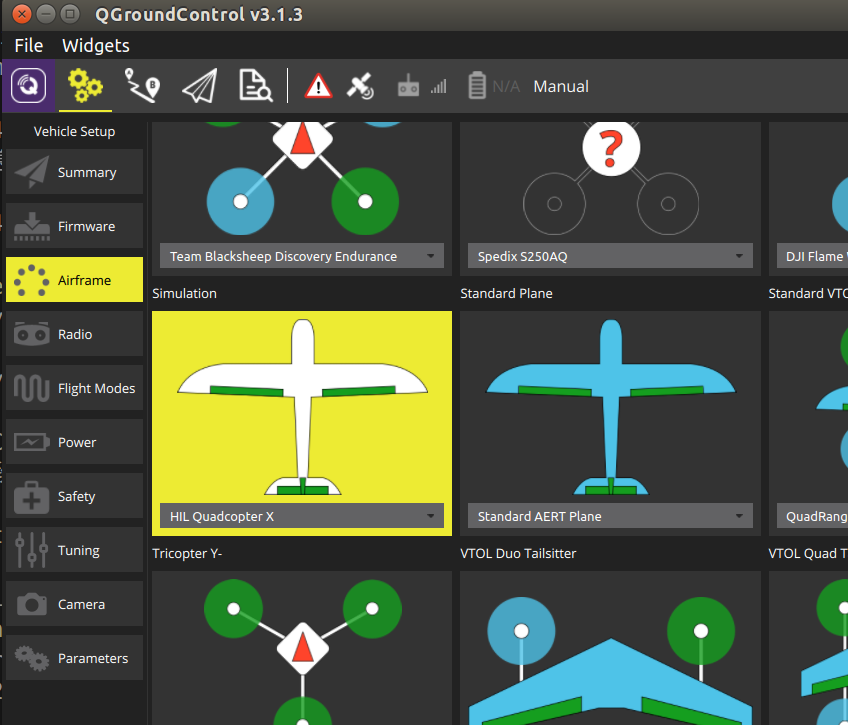
\includegraphics[width = 0.5\textwidth,trim = 0 -0 0 -0,clip]{HIL-2.png}	  
	\caption{\label{fig: HIL2} HIL模式时需要选择的机型}
\end{figure}
对应的系统参数应该是\texttt{SYS_AUTOSTART},选择HIL Quadcopter X时对应于1001:
\begin{figure}[htbp]
	\begin{minipage}[t]{0.5\textwidth}
	\centering
	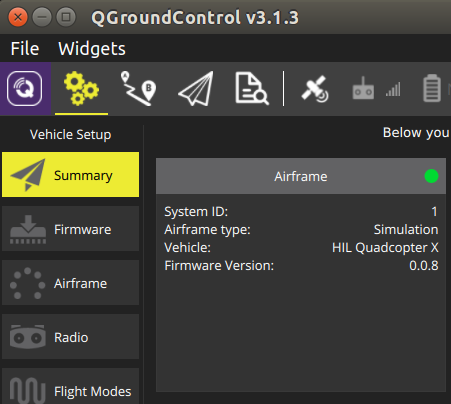
\includegraphics[width = 0.8\textwidth]{HIL-1.png}
	\caption{\label{fig:HIL1}HIL模式下的机型}
	\end{minipage}
	\begin{minipage}[t]{0.5\textwidth}
	\centering
	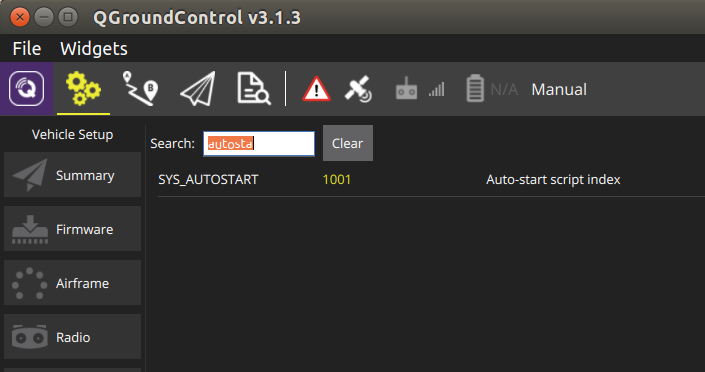
\includegraphics[width = 0.95\textwidth]{HIL-3.png}
	\caption{\label{fig:HIL3}HIL模式下对应的参数}
	\end{minipage}
\end{figure}

HIL在初始化时的启动文件也是\texttt{/firmware/ROMFS/px4fmu_common/init.d/rcS},其中会调用编译时生成的\texttt{/etc/init.d/rc.autostart}的文件。在这个rc.autostart文件中,通过比较\texttt{SYS_AUTOSTART}来确定执行\texttt{/etc/init.d/}文件夹下的机型脚本。1001对应于1001_rc_quad_x.hil,内容为:
\begin{lstlisting}[language=sh,numbers=left,firstnumber = 1,breaklines = true,numberstyle=\tiny,keywordstyle=\color{blue!70},commentstyle=\color{red!50!green!50!blue!50},frame=shadowbox, rulesepcolor=\color{red!20!green!20!blue!20}]
	#!nsh 
	#
	# @name HIL Quadcopter X
	#
	# @type Simulation
	#
	# @maintainer Anton Babushkin <anton@px4.io>
	#
	
	sh /etc/init.d/rc.mc_defaults
	
	set MIXER quad_x
	
	set HIL yes
\end{lstlisting}
主要参数是将\texttt{HIL}变量置为\texttt{yes},这个变量在rcS中的作用:(1)commander的启动方式为\texttt{"commander start -hil"};(2)启动\texttt{pwm_out_sim},且参数为\texttt{mode_pwm16}。pwm_out_sim的启动及其参数与SIL中的作用基本一致。commander采用hil模式时,会在线程中设置变量\texttt{startup_in_hil}
\begin{lstlisting}[language=C++,numbers=left,firstnumber = 0,breaklines = true,numberstyle=\tiny,keywordstyle=\color{blue!70},commentstyle=\color{red!50!green!50!blue!50},frame=shadowbox, rulesepcolor=\color{red!20!green!20!blue!20}]
	if (argc > 2) {
		if (!strcmp(argv[2],"-hil")) {
			startup_in_hil = true;
		} else {
			PX4_ERR("Argument %s not supported, abort.", argv[2]);
			thread_should_exit = true;
		}
	}
\end{lstlisting}
接着设置变量\texttt{status.hil_state}
\begin{lstlisting}[language=C++,numbers=left,firstnumber = 0,breaklines = true,numberstyle=\tiny,keywordstyle=\color{blue!70},commentstyle=\color{red!50!green!50!blue!50},frame=shadowbox, rulesepcolor=\color{red!20!green!20!blue!20}]
	if (startup_in_hil) {
		status.hil_state = vehicle_status_s::HIL_STATE_ON;
	} else {
		status.hil_state = vehicle_status_s::HIL_STATE_OFF;
	}
\end{lstlisting}
并在函数\texttt{set_control_mode}中:
\begin{lstlisting}[language=C++,numbers=left,firstnumber = 0,breaklines = true,numberstyle=\tiny,keywordstyle=\color{blue!70},commentstyle=\color{red!50!green!50!blue!50},frame=shadowbox, rulesepcolor=\color{red!20!green!20!blue!20}]
	control_mode.flag_system_hil_enabled = status.hil_state == vehicle_status_s::HIL_STATE_ON;
\end{lstlisting}
同时也会发布出去:
\begin{lstlisting}[language=C++,numbers=left,firstnumber = 0,breaklines = true,numberstyle=\tiny,keywordstyle=\color{blue!70},commentstyle=\color{red!50!green!50!blue!50},frame=shadowbox, rulesepcolor=\color{red!20!green!20!blue!20}]
	if (counter % (200000 / COMMANDER_MONITORING_INTERVAL) == 0 || status_changed) {
		set_control_mode();
		control_mode.timestamp = now;
		orb_publish(ORB_ID(vehicle_control_mode), control_mode_pub, &control_mode);
\end{lstlisting}
这个\texttt{vehicle_control_mode}会在sensors.cpp中的vehicle_control_mode_poll()函数中被订阅:
\begin{lstlisting}[language=C++,numbers=left,firstnumber = 1,breaklines = true,numberstyle=\tiny,keywordstyle=\color{blue!70},commentstyle=\color{red!50!green!50!blue!50},frame=shadowbox, rulesepcolor=\color{red!20!green!20!blue!20}]
void Sensors::vehicle_control_mode_poll()
{
	struct vehicle_control_mode_s vcontrol_mode;
	bool vcontrol_mode_updated;

	/* Check HIL state if vehicle control mode has changed */
	orb_check(_vcontrol_mode_sub, &vcontrol_mode_updated);

	if (vcontrol_mode_updated) {

		orb_copy(ORB_ID(vehicle_control_mode), _vcontrol_mode_sub, &vcontrol_mode);
		_armed = vcontrol_mode.flag_armed;

		/* switching from non-HIL to HIL mode */
		if (vcontrol_mode.flag_system_hil_enabled && !_hil_enabled) {
			_hil_enabled = true;
			_publishing = false;
			/* switching from HIL to non-HIL mode */

		} else if (!_publishing && !_hil_enabled) {
			_hil_enabled = false;
			_publishing = true;
		}
	}
}
\end{lstlisting}
其作用就是给变量\texttt{_publishing}赋值,而这个值在\texttt{Sensors::task_main()}中会决定是否将sensors中综合得到的传感器数据发布除去:
\begin{lstlisting}[language=C++,numbers=left,firstnumber = 1,breaklines = true,numberstyle=\tiny,keywordstyle=\color{blue!70},commentstyle=\color{red!50!green!50!blue!50},frame=shadowbox, rulesepcolor=\color{red!20!green!20!blue!20}]
if (_publishing && raw.timestamp > 0) {
	
				/* construct relative timestamps */
				if (_last_accel_timestamp[_accel.last_best_vote]) {
					raw.accelerometer_timestamp_relative = (int32_t)(_last_accel_timestamp[_accel.last_best_vote] - raw.timestamp);
				}
	
				if (_last_mag_timestamp[_mag.last_best_vote]) {
					raw.magnetometer_timestamp_relative = (int32_t)(_last_mag_timestamp[_mag.last_best_vote] - raw.timestamp);
				}
	
				if (_last_baro_timestamp[_baro.last_best_vote]) {
					raw.baro_timestamp_relative = (int32_t)(_last_baro_timestamp[_baro.last_best_vote] - raw.timestamp);
				}
	
				orb_publish(ORB_ID(sensor_combined), _sensor_pub, &raw);
\end{lstlisting}
综合来看,如果是HIL模式,sensors中的传感器数据不会发布到\texttt{sensor_combined}这个topic上,导航模块中订阅的传感器信息也就不是sensors发出的了。

实际在HIL模式中,从串口获取仿真数据并发布给导航的流程为:rcS启动串口的mavlink之后,也会订阅\texttt{vehicle_control_mode}这个topic,并设置\texttt{_hil_enabled = true},这样当\texttt{MavlinkReceiver::handle_message()}函数收到msg后,会在解析hil消息后并进行发布。在\texttt{MavlinkReceiver::handle_message_hil_sensor()}函数中,会将数据发布到\texttt{sensor_gyro}等传感器数据以及\texttt{sensor_combined}这个导航使用的topic中。

而在HIL模式中,将飞控数据用mavlink协议从串口发送的流程为:mavlink 启动后会生成一个MavLinkStream链表,在mavlink_main.cpp中的\texttt{int Mavlink::task_main()}函数中,会执行:
\begin{lstlisting}[language=C++,numbers=left,firstnumber = 1,breaklines = true,numberstyle=\tiny,keywordstyle=\color{blue!70},commentstyle=\color{red!50!green!50!blue!50},frame=shadowbox, rulesepcolor=\color{red!20!green!20!blue!20}]
/* update streams */
MavlinkStream *stream;
LL_FOREACH(_streams, stream) {
	stream->update(t);
}
\end{lstlisting}
这样就会在链表中调用每一个stream节点的update()成员函数。在update()函数中,会判断当前时间是否超过了上次发送后的间隔,然后调用send(t)进行数据发送。

综合来看,在HIL模式下数据的接收与发送都是通过mavlink相关的模块来实现的,而SIL中则是用simulator实现数据中转的。

另外要注意的是,虽然sensors不发布\texttt{sensor_combined}这个topic,但是sensors以及其他的传感器模块(mpu6000等)的线程仍然在进行,所以传感器数据(HIL时飞控板的真实传感器数据)仍然会读取并在sensors中订阅,所以如果在nsh中用\texttt{sensors status}命令查看状态,依然会出现多个传感器的数据:
\begin{figure}[htbp]
	\figskip
	\centering
	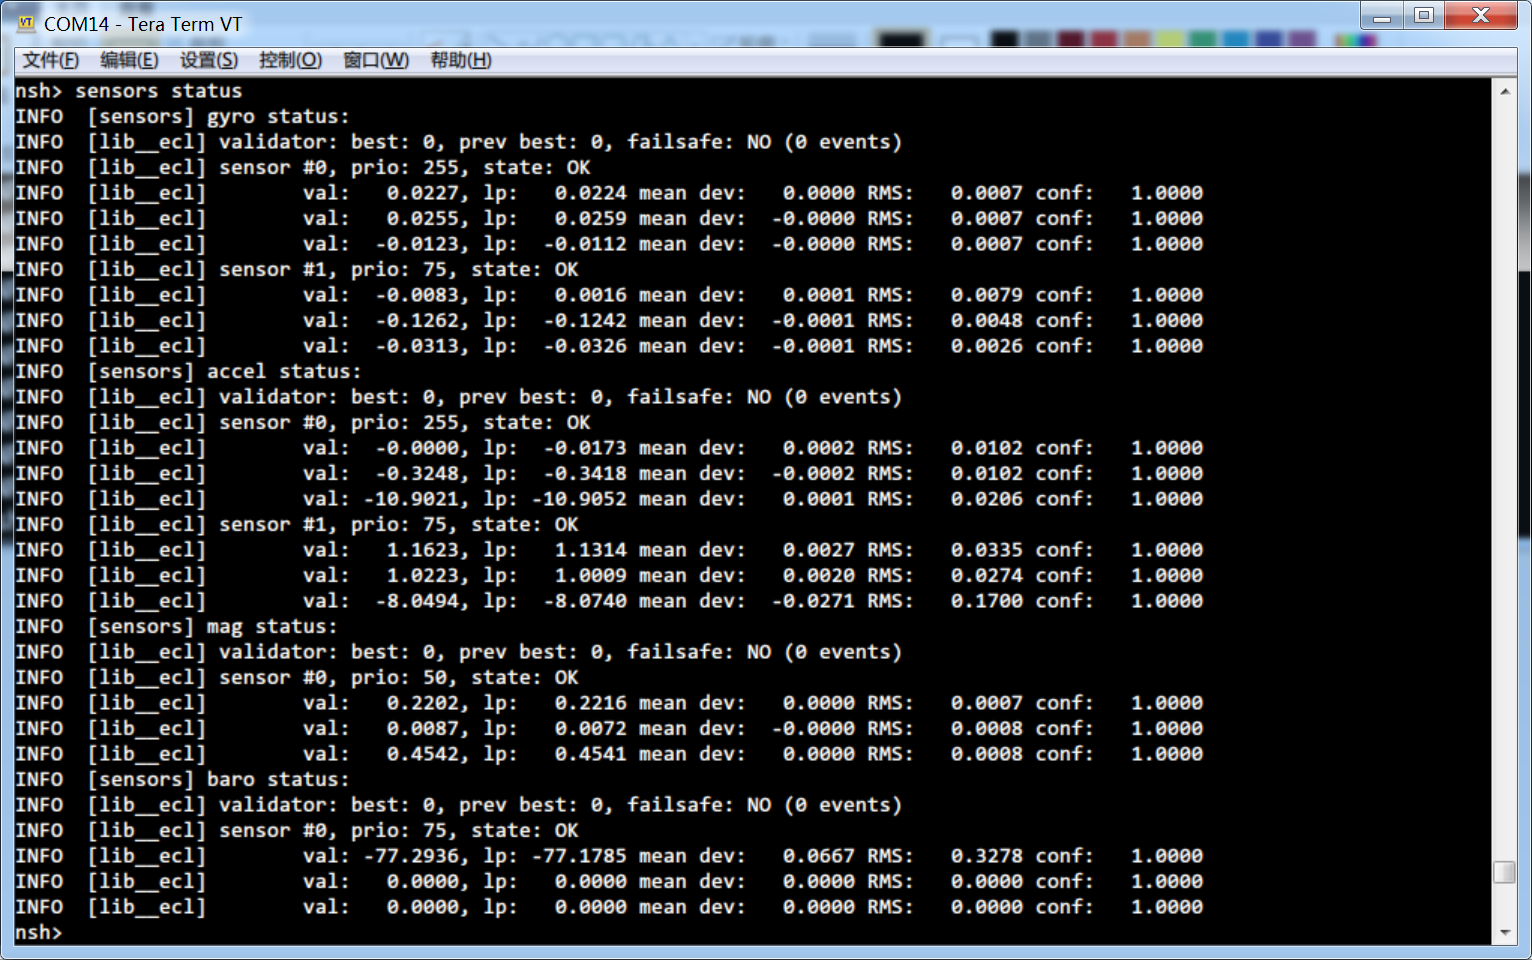
\includegraphics[width = 0.75\textwidth,trim = 0 -0 0 -0,clip]{nsh-0.png}	  
	\caption{\label{fig: sensors0} HIL模式下飞控通电,未连接jMAVSim时的sensors status}
\end{figure}

\begin{figure}[htbp]
	\figskip
	\centering
	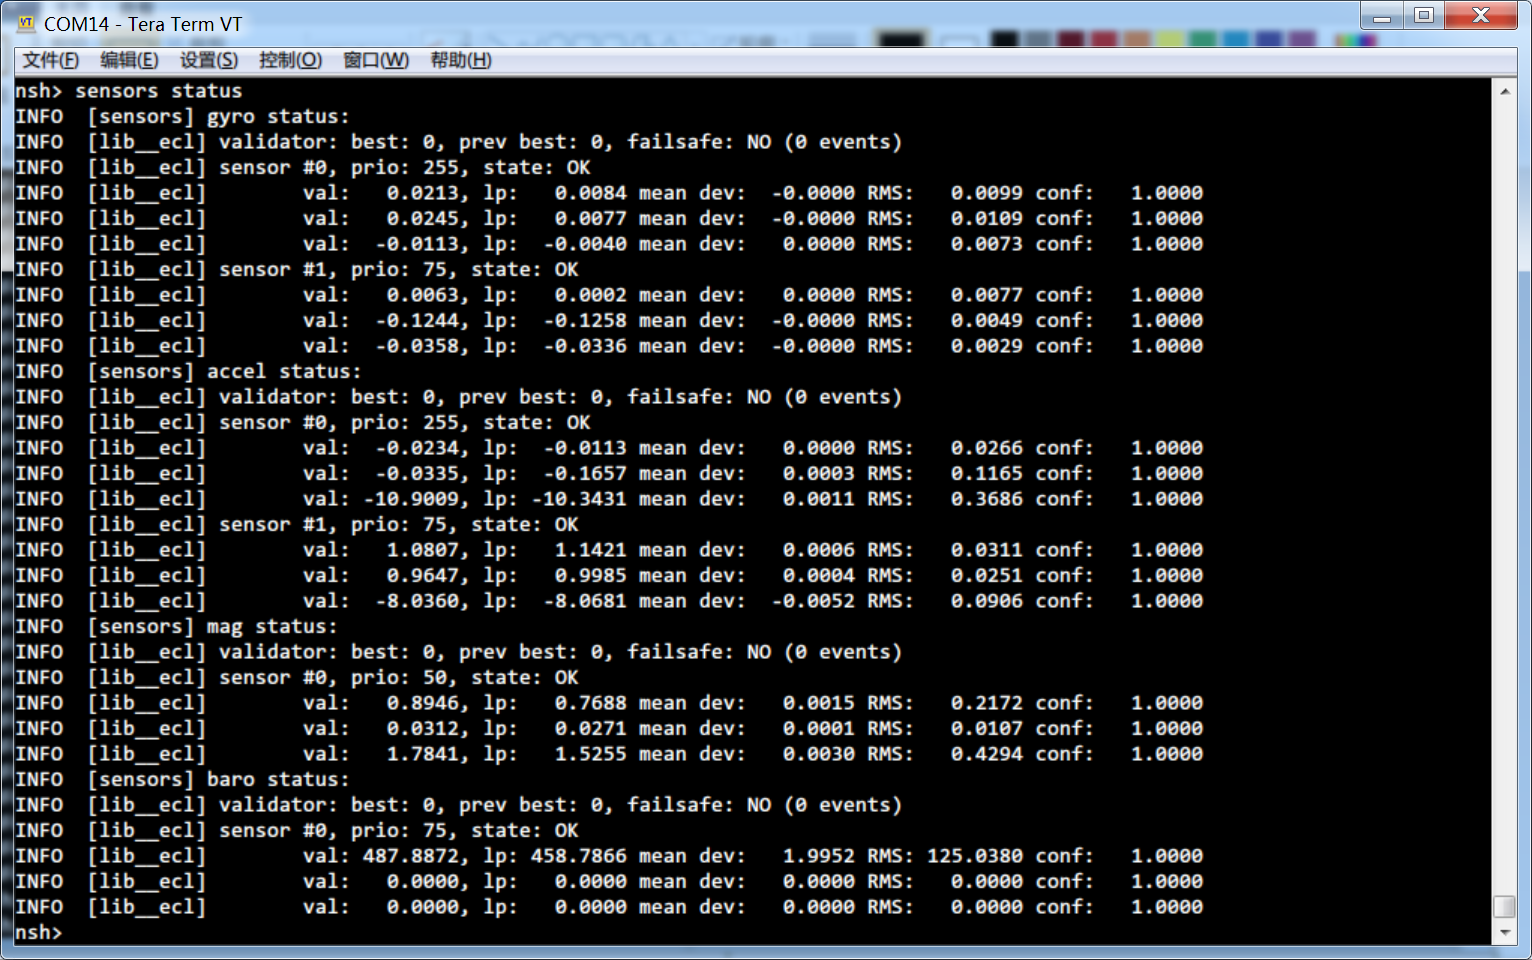
\includegraphics[width = 0.75\textwidth,trim = 0 -0 0 -0,clip]{nsh-0-hil.png}	  
	\caption{\label{fig: sensors1} HIL模式下飞控通电,连接jMAVSim之后的sensors status}
\end{figure}
从上面的图\ref{fig: sensors0}和图\ref{fig: sensors1}可知,确实能够读到多个传感器数据,并且连接jMAVSim之后默认的传感器数据都是仿真数据。而\texttt{baro}气压计状态更清晰的说明,未连接jMAVSim或jMAVSim没发数据的时候,\texttt{sensors status}的读数是飞控的真实数据。

进一步分析可知,由于真实传感器以及MavlinkReceiver中发布数据都是按照单传感器模式(\texttt{orb_advertise()}, 则优先级为默认值75)发布,所以两者的数据会发生重叠,这样即使真实气压计和jMAVSim都有baro数据,但\texttt{sensors status}中baro只有一个数据。所以如果在\texttt{void MavlinkReceiver::handle_message_hil_sensor(mavlink_message_t *msg)}函数中使用\texttt{orb_advertise_multi()}进行声明优先级为100(\texttt{ORB_PRIO_HIGH}),就能够显示多个baro数据了:
\begin{lstlisting}[language=C++,numbers=left,firstnumber = 1,breaklines = true,numberstyle=\tiny,keywordstyle=\color{blue!70},commentstyle=\color{red!50!green!50!blue!50},frame=shadowbox, rulesepcolor=\color{red!20!green!20!blue!20}]
	/* baro */
	{
		struct baro_report baro = {};

		baro.timestamp = timestamp;
		baro.pressure = imu.abs_pressure;
		baro.altitude = imu.pressure_alt;
		baro.temperature = imu.temperature;
		int a = -1;
		if (_baro_pub == nullptr) {
			// _baro_pub = orb_advertise(ORB_ID(sensor_baro), &baro);
			_baro_pub = orb_advertise_multi(ORB_ID(sensor_baro), &baro, &a, ORB_PRIO_HIGH);

		} else {
			orb_publish(ORB_ID(sensor_baro), _baro_pub, &baro);
		}
	}
\end{lstlisting}

\begin{figure}[htbp]
	\figskip
	\centering
	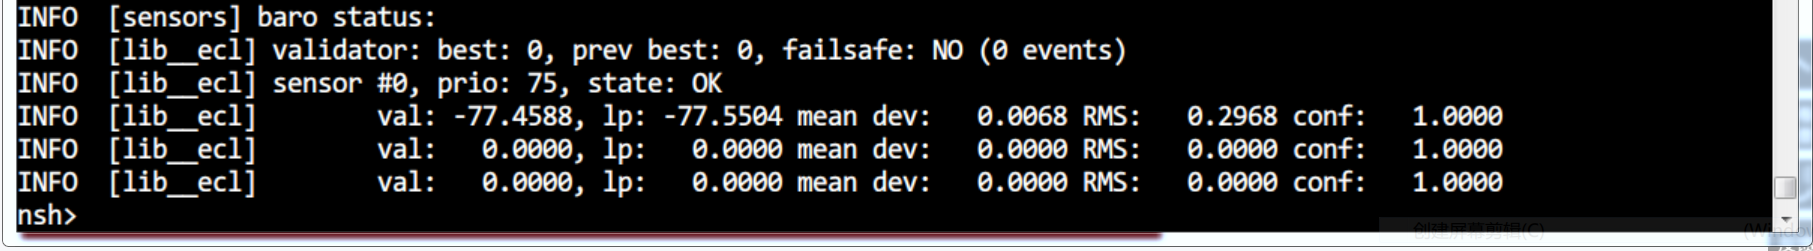
\includegraphics[width = 0.9\textwidth,trim = 0 -0 0 -0,clip]{nsh-1.png}	  
	\caption{\label{fig: sensors2} HIL模式下飞控通电,未连接jMAVSim时的baro}
\end{figure}

\begin{figure}[htbp]
	\figskip
	\centering
	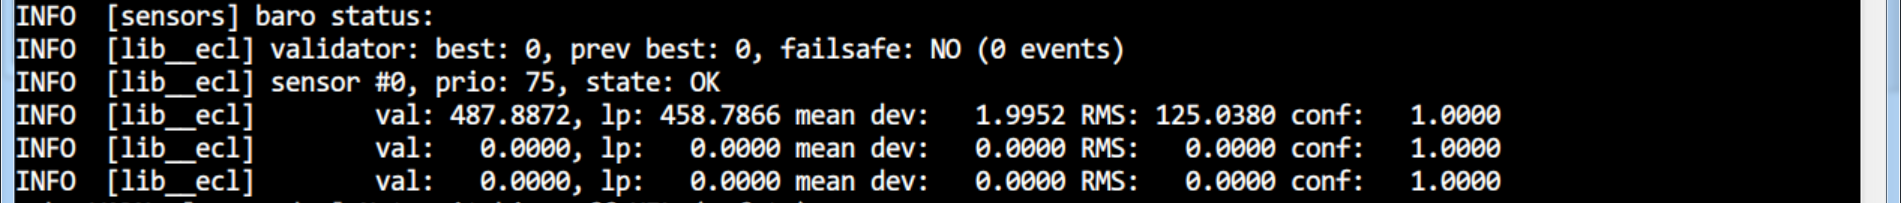
\includegraphics[width = 0.9\textwidth,trim = 0 -0 0 -0,clip]{nsh-2.png}	  
	\caption{\label{fig: sensors3} HIL模式下飞控通电,连接jMAVSim之后的baro}
\end{figure}

\begin{figure}[htbp]
	\figskip 
	\centering
	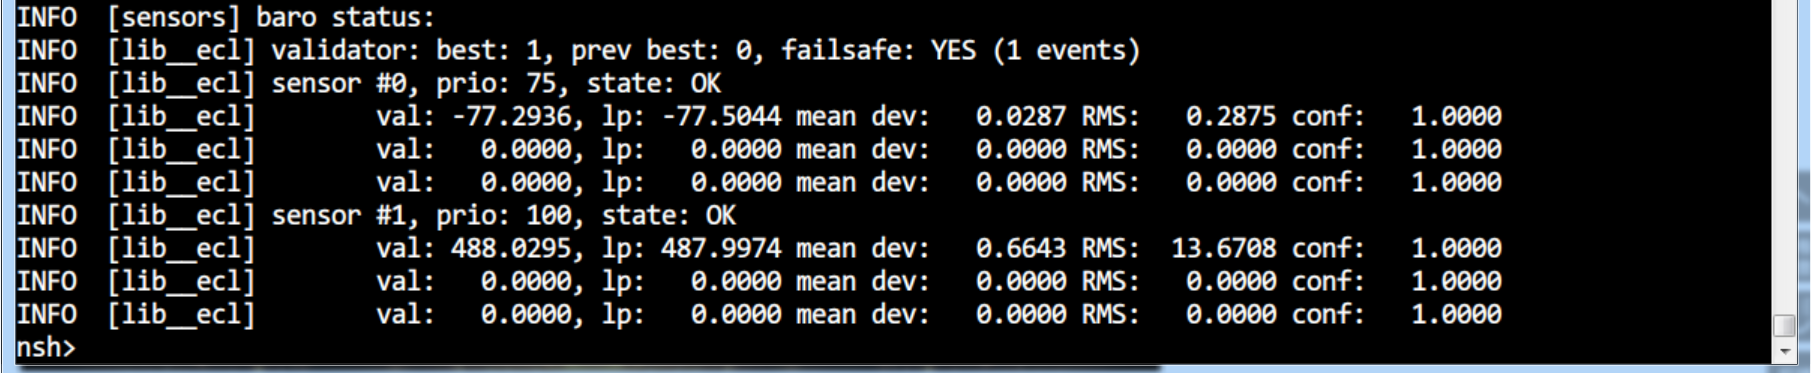
\includegraphics[width = 0.9\textwidth,trim = 0 -0 0 -0,clip]{nsh-3.png}	  
	\caption{\label{fig: sensors4} 增加优先级后,连接jMAVSim之后的baro}
\end{figure}

\subsection{jMAVSim启动时间的讨论}
虽然\href{http://www.pixhawk.com/dev/hil/jmavsim#hardware_in_the_loop_hitl}{官网教程}中介绍了HIL模式的连接方式,但是对于飞控上电和jMAVSim开启的先后并没有说明。按照字面正常推断,应该是飞控首先上电,然后在PC端打开jMAVSim软件(如果先开启jMAVSim的话,由于串口没有数据通信,jMAVSim会自动关闭)。

这里就存在一个飞控上电与jMAVSim启动间隔时间的问题。经过测试,采用INAV导航算法时,如果在一定时间之后才启动jMAVSim(向PX4发送数据)的话,飞控将不能锁定HOME点坐标。对应的现象是能够获取初始GPS,但无法定位当前飞控坐标,也无法响应mission等指令。原因如下:

在\texttt{position_estimator_inav_main.cpp}中,飞控上电后会启动导航主线程\texttt{position_estimator_inav_thread_main}。与其他的常规主线程类似,在阻塞等待数据更新这个主循环之前,是对导航状态量的初始化过程。而这个初始化流程的最后一步是等待并采集一定数量的气压高数据,最后确定气压高偏移值,并将\texttt{local_pos.z_valid} 置为真。那如果jMAVSim一直为发送气压数据,经过一定的等待时间(\texttt{MAX_WAIT_FOR_BARO_SAMPLE=3s})后,也会结束等待气压数据,而这时\texttt{local_pos.z_valid}仍为假。具体代码如下。
\begin{lstlisting}[language=C++,numbers=left,firstnumber = 1,breaklines = true,numberstyle=\tiny,keywordstyle=\color{blue!70},commentstyle=\color{red!50!green!50!blue!50},frame=shadowbox, rulesepcolor=\color{red!20!green!20!blue!20}]
while (wait_baro && !thread_should_exit) {
	int ret = px4_poll(&fds_init[0], 1, 1000);

	if (ret < 0) {
		/* poll error */
		mavlink_log_info(&mavlink_log_pub, "[inav] poll error on init");

	} else if (hrt_absolute_time() - baro_wait_for_sample_time > MAX_WAIT_FOR_BARO_SAMPLE) {
		wait_baro = false;
		mavlink_log_info(&mavlink_log_pub, "[inav] timed out waiting for a baro sample");

	} else if (ret > 0) {
		if (fds_init[0].revents & POLLIN) {
			orb_copy(ORB_ID(sensor_combined), sensor_combined_sub, &sensor);

			if (wait_baro && sensor.timestamp + sensor.baro_timestamp_relative != baro_timestamp) {
				baro_timestamp = sensor.timestamp + sensor.baro_timestamp_relative;
				baro_wait_for_sample_time = hrt_absolute_time();

				/* mean calculation over several measurements */
				if (baro_init_cnt < baro_init_num) {
					if (PX4_ISFINITE(sensor.baro_alt_meter)) {
						baro_offset += sensor.baro_alt_meter;
						baro_init_cnt++;
					}

				} else {
					wait_baro = false;
					baro_offset /= (float) baro_init_cnt;
					local_pos.z_valid = true;
					local_pos.v_z_valid = true;
				}
			}
		}

	} else {
		PX4_WARN("INAV poll timeout");
	}
}
\end{lstlisting}

最后发布\texttt{vehicle_global_position}消息时的判别条件是\texttt{if (local_pos.xy_global \&\& local_pos.z_global)}。显然jMAVSim启动时间会影响到这里的消息发布。所以即便之后飞控收到了GPS数据,但\texttt{vehicle_global_position}也始终无法发布,之后也就会遇到前文中出现的现象了。



% \begin{lstlisting}[language=C++,numbers=left,firstnumber = 0,breaklines = true,numberstyle=\tiny,keywordstyle=\color{blue!70},commentstyle=\color{red!50!green!50!blue!50},frame=shadowbox, rulesepcolor=\color{red!20!green!20!blue!20}]
% \end{lstlisting}





















\cleardoublepage
